\documentclass[twocolumn,twoside,11pt,a4paper]{article}

\usepackage[portuguese]{babel}  % portuguese
\usepackage{graphicx}           % images: .png or .pdf w/ pdflatex; .eps w/ latex

\usepackage{lipsum}             % generate dummy text throughout this template

%% For iso-8859-1 (latin1), comment next line and uncomment the second line
\usepackage[utf8]{inputenc}
%\usepackage[latin1]{inputenc}

\usepackage[T1]{fontenc}        % T1 fonts
\usepackage{lmodern}            % fonts
\usepackage[sc]{mathpazo}       % Use the Palatino font
\linespread{1.05}               % Line spacing - Palatino needs more space between lines
\usepackage{microtype}          % Slightly tweak font spacing for aesthetics
\usepackage{url}                % urls
\usepackage[hang, small, labelfont=bf,up,textfont=it,up]{caption} % Custom captions under/above floats in tables or figures
\usepackage{booktabs}           % Horizontal rules in tables
\usepackage{float}              % Required for tables and figures in the multi-column environment - they need to be placed in specific locations with the [H] (e.g. \begin{table}[H])
\usepackage{paralist}           % Used for the compactitem environment which makes bullet points with less space between them

% geometry package
\usepackage[outer=20mm,inner=20mm,vmargin=15mm,includehead,includefoot,headheight=15pt]{geometry}
%% space between columns
\columnsep 10mm

\usepackage{abstract}           % Allows abstract customization
\renewcommand{\abstractnamefont}{\normalfont\bfseries} % Set the "Abstract" text to bold
\renewcommand{\abstracttextfont}{\normalfont\small\itshape} % Set the abstract itself to small italic text

% \usepackage{titlesec}           % Allows customization of titles
% \renewcommand\thesection{\Roman{section}} % Roman numerals for the sections
% \renewcommand\thesubsection{\Roman{subsection}} % Roman numerals for subsections
% \titleformat{\section}[block]{\large\scshape\centering}{\thesection.}{1em}{} % Change the look of the section titles
% \titleformat{\subsection}[block]{\large}{\thesubsection.}{1em}{} % Change the look of the section titles

\usepackage[pdftex]{hyperref}
\hypersetup{%
    a4paper = true,              % use A4 paper 
    bookmarks = true,            % make bookmarks 
    colorlinks = true,           % false: boxed links; true: colored links
    pdffitwindow = false,        % page fit to window when opened
    pdfpagemode = UseNone,       % do not show bookmarks
    pdfpagelayout = SinglePage,  % displays a single page
    pdfpagetransition = Replace, % page transition
    linkcolor=blue,              % hyperlink colors
    urlcolor=blue,
    citecolor=blue,
    anchorcolor=green
}

\usepackage{indentfirst}         % indent also 1st paragraph

\usepackage{fancyhdr}            % Headers and footers
\pagestyle{fancy}                % pages have headers and footers
\fancyhead{}                     % Blank out the default header
\fancyfoot{}                     % Blank out the default footer
\fancyhead[LO,RE]{Exemplo de artigo em \LaTeX} % Custom header text
\fancyhead[RO,LE]{\thepage}      % Custom header text
\fancyfoot[RO,LE]{Grupo xx, \today} % Custom footer text
\renewcommand{\headrulewidth}{0.4pt}
\renewcommand{\footrulewidth}{0.4pt}

%\hyphenation{}                  % explicit hyphenation

%----------------------------------------------------------------------------------------
%	macro definitions
%----------------------------------------------------------------------------------------

% entities
\newcommand{\class}[1]{{\normalfont\slshape #1\/}}
\newcommand{\svg}{\class{SVG}}
\newcommand{\scada}{\class{SCADA}}
\newcommand{\scadadms}{\class{SCADA/DMS}}

%----------------------------------------------------------------------------------------
%	TITLE SECTION
%----------------------------------------------------------------------------------------

\title{\vspace{-15mm}\fontsize{24pt}{10pt}\selectfont\textbf{Article Title}} % Article title

\author{First Author\\
\small \texttt{first@school.edu}\\
\and
Second Author\\
\small \texttt{noremembers@school.edu}
\vspace{-5mm}
}

\date{\today}

%----------------------------------------------------------------------------------------

\begin{document}

\maketitle
\thispagestyle{plain}            % no headers in the first page

%----------------------------------------------------------------------------------------
%	ABSTRACT
%----------------------------------------------------------------------------------------

\begin{abstract}
O \svg{} é uma linguagem XML que descreve gráficos de duas dimensões.
A tecnologia \svg{} é usada aqui para representar sinópticos e
permitir a interação do utilizador do sistema através de uma
interface Web.  \lipsum[1]
\end{abstract}

%----------------------------------------------------------------------------------------
%	ARTICLE CONTENTS
%----------------------------------------------------------------------------------------

\section{Introdução}\label{sec:intro}

Os sistemas \scada{} (\emph{Supervisory Control And Data Acquisition})
são responsáveis pela recolha e análise de informação em tempo real.
Atualmente estes sistemas recorrem às mais avançadas tecnologias de
computação e comunicação para monitorizar e controlar estruturas ou
equipamentos industriais dispersos geograficamente e recorrem a
interfaces gráficas para tornar a interação com o utilizador mais
amigável\footnote{Exemplo de artigo retirado de uma submissão à
  Conferência XATA2006, mas sem usar LLNCS.}.

\lipsum[2]

Para além desta introdução, onde se caracterizou o problema abordado
por este projeto, refere-se na Secção~\ref{sec:sota} o
estado da arte e são descritos os trabalhos relacionados com a
visualização de diagramas sinópticos de sistemas \scada{} na
\textit{Web}. 

%------------------------------------------------

\section{\svg}\label{sec:sota}

Nos últimos tempos têm surgido diversas soluções, apresentadas por
empresas do sector Automação de Sistemas para a disponibilização de
sistemas \scadadms{} na \textit{Web}.

\emph{Scalable Vector Graphics} é uma linguagem em formato XML que
descreve gráficos de duas dimensões. 
Este formato padronizado pela W3C (\emph{World Wide Web Consortium})
é livre de patentes ou direitos de autor e está totalmente
documentado, à semelhança de outros W3C standards~\cite{kn:svgdoc}.

Sendo uma linguagem XML, o \svg{} herda uma série de vantagens: a
possibilidade de transformar \svg{} usando técnicas como XSLT, de embeber
\svg{} em qualquer documento XML usando \textit{namespaces} ou até de 
estilizar \svg{} recorrendo a CSS (\emph{Cascade Style Sheets}). 
De uma forma geral, pode dizer-se que \svg{}s interagem bem com as
atuais tecnologias ligadas ao XML e à Web, tal como referido
em~\cite{kn:svgibm,kn:svgw3c}.

\subsection{Batik \svg{} Toolkit} \label{batik} 

Batik é um conjunto de bibliotecas baseadas em \textit{Java} que
permitem o uso de imagens \svg{} (visualização, geração ou
manipulação) em aplicações ou \textit{applets} \cite{kn:batikarchitecture}.  
O projeto Batik destina-se a fornecer ao programador alguns módulos
que permitem desenvolver soluções especificas usando \svg. 

\lipsum[3]

%------------------------------------------------

\section{Visualizador de Sinópticos}\label{sec:application}

A arquitetura do visualizador assenta sobre os seguintes conceitos base \cite{kn:zpmd}:
\begin{compactitem}
\item \textbf{Componentes} --- Suspendisse auctor mattis augue \emph{push};
\item \textbf{Praesent} --- Sit amet sem maecenas eleifend facilisis leo;
\item \textbf{Pellentesque} --- Habitant morbi tristique senectus et netus.
\end{compactitem}

\lipsum[4]

Apresenta-se de seguida um exemplo de equação, completamente fora do contexto:
\begin{eqnarray}
CIF_1: \hspace*{5mm}F_0^j(a) &=& \frac{1}{2\pi \iota} \oint_{\gamma} \frac{F_0^j(z)}{z - a} dz\\
CIF_2: \hspace*{5mm}F_1^j(a) &=& \frac{1}{2\pi \iota} \oint_{\gamma} \frac{F_0^j(x)}{x - a} dx \label{eq:cif}
\end{eqnarray}

Na Equação~\ref{eq:cif} \lipsum[5]

\subsection{Exemplo de Figura}

É apresentado na Figura~\ref{fig:arch} %da página~\pageref{fig:arch}
um exemplo de figura flutuante que ficará onde o \LaTeX\ entender.

\begin{figure}
  \begin{center}
    \leavevmode
    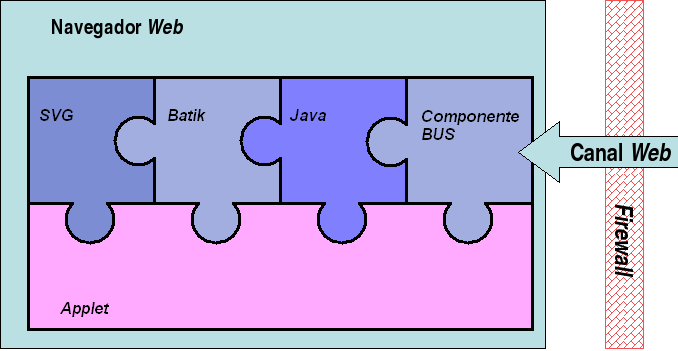
\includegraphics[width=0.45\textwidth]{puzzle}
    \caption{Arquitetura da Solução Proposta}
    \label{fig:arch}
  \end{center}
\end{figure}

\lipsum[6]

\subsection{Exemplo de Tabela}

É apresentado na Tabela~\ref{tab:exemplo1} um exemplo de tabela.

\begin{table}[H]
  \centering
  \caption{Uma Tabela Simples}
  \begin{tabular}{| l | p{45mm} |}
    \hline
    \textbf{Acrónimo} & \textbf{Significado}\\
    \hline
    \hline
    ADT   & \emph{Abstract Data Type}\\\hline
    ANDF  & \emph{Architecture-Neutral Distribution Format}\\\hline
    API   & \emph{Application Programming Interface}\\
    \hline
  \end{tabular}
  \label{tab:exemplo1}
\end{table}

\lipsum[7]

% \begin{table}
%   \centering
%   \caption{Tabela Exemplo}
% \begin{tabular}{|c|r@{.}lr@{.}lr@{.}l||r|}
% 	\hline
% \multicolumn{8}{|c|}
% 	{\rule[-3mm]{0mm}{8mm}Iteração $k$ de $f(x_n)$} \\
% \textbf{\em k}
% 	& \multicolumn{2}{c}{$x_1^k$}
% 	& \multicolumn{2}{c}{$x_2^k$}
% 	& \multicolumn{2}{c||}{$x_3^k$}
% 	& comentários \\ \hline \hline
% 0   & -0&3                 & 0&6                 &  0&7   & - \\
% 1   &  0&47102965 & 0&04883157 & -0&53345964  & $\delta<\epsilon$ \\
% 2   &  0&49988691 & 0&00228830 & -0&52246185  & $\delta < \varepsilon$ \\
% 3   &  0&49999976 & 0&00005380 & -0&523656   &   $N$ \\
% 4   &  0&5                 & 0&00000307 & -0&52359743  & \\
% \vdots	& \multicolumn{2}{c}{\vdots}
% 	& \multicolumn{2}{c}{$\ddots$}
% 	& \multicolumn{2}{c||}{\vdots}  & \\
% 7   &  0&5   & 0&0    & \textbf{-0}&\textbf{52359878}
% 		 & $\delta<10^{-8}$ \\ \hline
% \end{tabular}
%   \label{tab:exemplo2}
% \end{table}

%------------------------------------------------

\section{Conclusões}\label{sec:conclusions}

Neste artigo abordou-se o desenvolvimento de um protótipo, com vista a
estudar a adequadibilidade da tecnologia \svg{} à visualização de
sinópticos na \textit{Web}.

\lipsum[8]

%----------------------------------------------------------------------------------------
%	REFERENCE LIST
%----------------------------------------------------------------------------------------

%% auto bibliographic list 
\renewcommand{\bibname}{Referências}
% uses bibtex file
%\bibliographystyle{alpha-pt}
%\bibliographystyle{alpha}
\bibliographystyle{unsrt-pt}
%\bibliographystyle{unsrt}
\bibliography{artigo}

%----------------------------------------------------------------------------------------

\end{document}


